\documentclass{article}

\usepackage{tikz}
\usetikzlibrary{calc}
\begin{document}
\begin{figure}
\tikzset{
tick/.style = {black, very thick}
}

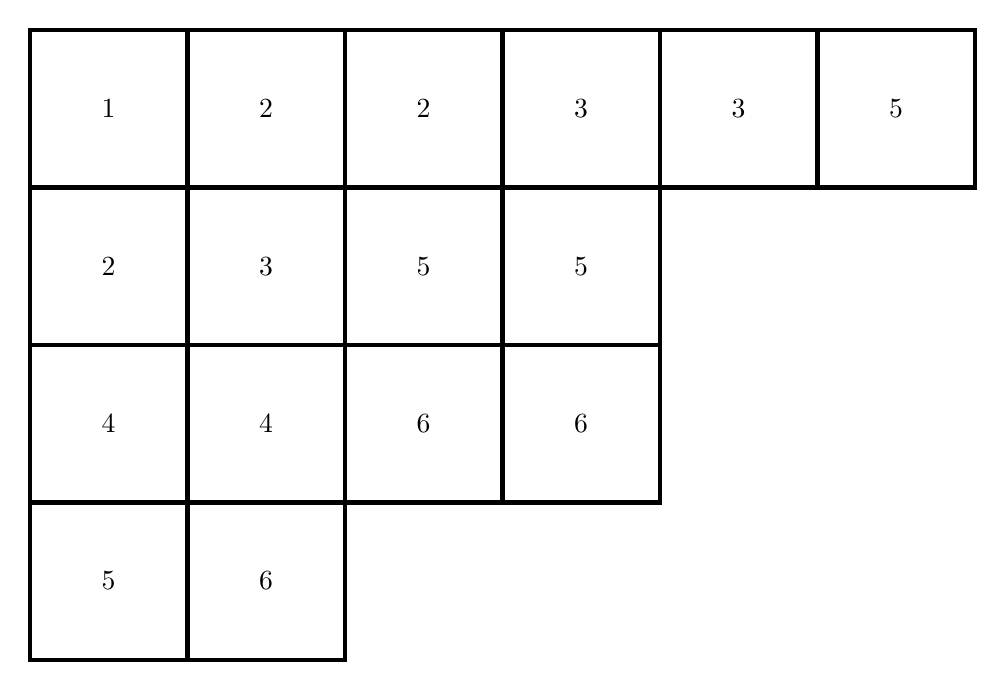
\begin{tikzpicture} % boxlength=2%ZEILE NR. 0 (von unten)

%ELEMENT IN SPALTE NR. 0 (von links)
\draw [ultra thick] (0,0) rectangle (2,2);
\node at ($(1.0,1.0)$) {$5$};

%ELEMENT IN SPALTE NR. 1 (von links)
\draw [ultra thick] (2,0) rectangle (4,2);
\node at ($(3.0,1.0)$) {$6$};




%ZEILE NR. 1 (von unten)

%ELEMENT IN SPALTE NR. 0 (von links)
\draw [ultra thick] (0,2) rectangle (2,4);
\node at ($(1.0,3.0)$) {$4$};

%ELEMENT IN SPALTE NR. 1 (von links)
\draw [ultra thick] (2,2) rectangle (4,4);
\node at ($(3.0,3.0)$) {$4$};

%ELEMENT IN SPALTE NR. 2 (von links)
\draw [ultra thick] (4,2) rectangle (6,4);
\node at ($(5.0,3.0)$) {$6$};

%ELEMENT IN SPALTE NR. 3 (von links)
\draw [ultra thick] (6,2) rectangle (8,4);
\node at ($(7.0,3.0)$) {$6$};




%ZEILE NR. 2 (von unten)

%ELEMENT IN SPALTE NR. 0 (von links)
\draw [ultra thick] (0,4) rectangle (2,6);
\node at ($(1.0,5.0)$) {$2$};

%ELEMENT IN SPALTE NR. 1 (von links)
\draw [ultra thick] (2,4) rectangle (4,6);
\node at ($(3.0,5.0)$) {$3$};

%ELEMENT IN SPALTE NR. 2 (von links)
\draw [ultra thick] (4,4) rectangle (6,6);
\node at ($(5.0,5.0)$) {$5$};

%ELEMENT IN SPALTE NR. 3 (von links)
\draw [ultra thick] (6,4) rectangle (8,6);
\node at ($(7.0,5.0)$) {$5$};




%ZEILE NR. 3 (von unten)

%ELEMENT IN SPALTE NR. 0 (von links)
\draw [ultra thick] (0,6) rectangle (2,8);
\node at ($(1.0,7.0)$) {$1$};

%ELEMENT IN SPALTE NR. 1 (von links)
\draw [ultra thick] (2,6) rectangle (4,8);
\node at ($(3.0,7.0)$) {$2$};

%ELEMENT IN SPALTE NR. 2 (von links)
\draw [ultra thick] (4,6) rectangle (6,8);
\node at ($(5.0,7.0)$) {$2$};

%ELEMENT IN SPALTE NR. 3 (von links)
\draw [ultra thick] (6,6) rectangle (8,8);
\node at ($(7.0,7.0)$) {$3$};

%ELEMENT IN SPALTE NR. 4 (von links)
\draw [ultra thick] (8,6) rectangle (10,8);
\node at ($(9.0,7.0)$) {$3$};

%ELEMENT IN SPALTE NR. 5 (von links)
\draw [ultra thick] (10,6) rectangle (12,8);
\node at ($(11.0,7.0)$) {$5$};







\end{tikzpicture}
\end{figure}
\end{document}

